\documentclass[tikz, margin = 1cm] {standalone}

\begin{document}
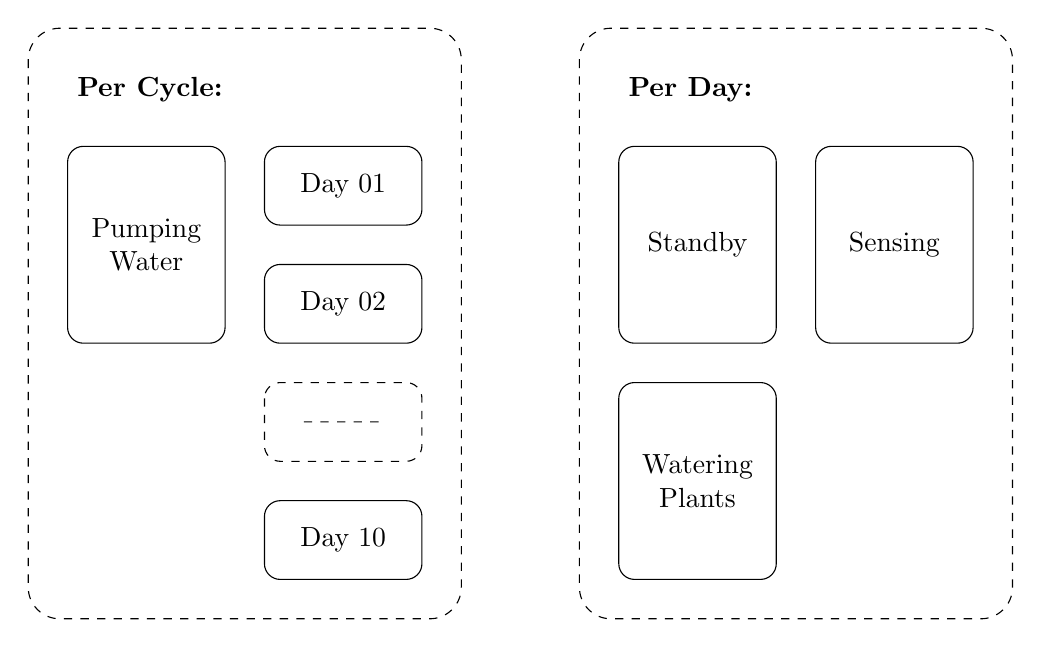
\begin{tikzpicture}

    \draw [rounded corners = 4mm, dashed]
    (0,0) rectangle ++(5.5,-7.5)
    (0,0)
    coordinate (cycleStart)
    ;

    \draw
    (cycleStart)
    ++(0.5,-0.5)
    node [align = center, anchor = north west] {\textbf{Per Cycle:}}
    ++(0,-1.0)
    coordinate (pumpStart)
    ;

    \draw [rounded corners = 2mm]
    (pumpStart) rectangle +(2,-2.5)

    ++(1,-1.25)
    node [align = center, anchor = center] {Pumping \\ Water}
    ++(-1,1.25)

    ++(2.5,0)
    coordinate (dayStart)
    ;

    \foreach \i in {1,...,2} {
        \draw [rounded corners = 2mm]
        (dayStart) rectangle +(2,-1)

        ++(1,-0.5)
        node [align = center, anchor = center] {Day 0\i}
        ++(-1,0.5)

        ++(0, -1.5)
        coordinate (dayStart)
        ;
    }

    \draw [rounded corners = 2mm, dashed]
    (dayStart) rectangle +(2,-1)
    ++(0.5,-0.5) -- +(1,0)
    ++(-0.5, -1.0)
    coordinate (dayStart)

    ;

    \draw [rounded corners = 2mm]
    (dayStart) rectangle +(2,-1)

    ++(1,-0.5)
    node [align = center, anchor = center] {Day 10}
    ++(-1,0.5)

    ++(0, -1.5)
    coordinate (dayStart)
    ;

    %% Drawing Per Day Power Consumption Diagram
    \draw
    (0,0) ++(5.5,0)
    ++(1.5,0)
    coordinate (perdayStart)
    ;

    \draw [rounded corners = 4mm, dashed]
    (perdayStart) rectangle ++(5.5,-7.5)
    ;

    \draw
    (perdayStart)
    ++(0.5,-0.5)
    node [align = center, anchor = north west] {\textbf{Per Day:}}
    ++(0,-1.0)
    coordinate (standbyStart)
    ;

    %% Drawing Stand by
    \draw [rounded corners = 2mm]
    (standbyStart) rectangle +(2,-2.5)

    ++(1,-1.25)
    node [align = center, anchor = center] {Standby}
    ++(-1,1.25)

    ++(2.5,0)
    coordinate (sensingStart)
    ;

    %% Drawing sensing
    \draw [rounded corners = 2mm]
    (sensingStart) rectangle +(2,-2.5)

    ++(1,-1.25)
    node [align = center, anchor = center] {Sensing}
    ++(-1,1.25)

    ++(-2.5,-3.0)
    coordinate (wateringStart)
    ;

    %% Drawing Stand by
    \draw [rounded corners = 2mm]
    (wateringStart) rectangle +(2,-2.5)

    ++(1,-1.25)
    node [align = center, anchor = center] {Watering \\ Plants}
    ++(-1,1.25)

    ++(2.5,0)
    coordinate (tmp)
    ;

    %% Drawing the arrow from day 01 to perday
    %% \draw [dashed, -stealth, white!60!black]

    %% (pumpStart-|dayStart)
    %% ++(0,-0.5)
    %% coordinate (arrowHeight)

    %% (arrowHeight)
    %% ++(2.1,0)
    %% coordinate (arrowStart)

    %% (arrowHeight-|perdayStart)
    %% ++(-0.1,0)
    %% coordinate (arrowEnd)

    %% (arrowStart) -- (arrowEnd)
    %% ;

\end{tikzpicture}
\end{document}
